\documentclass{article}
\usepackage[a4paper, margin=5em]{geometry}
\usepackage{fancyhdr}
\usepackage{lastpage}
\usepackage{graphicx}
\usepackage{hyperref}
%\usepackage{ngerman}
\usepackage{babel}
\usepackage{enumitem}
\usepackage{csquotes}
\usepackage{caption}
\usepackage{fancyvrb}
\usepackage{minted}

\newcommand{\gqq}[1]{\glqq{}#1\grqq{}}

\pagestyle{fancy}
\fancyhf{}
\renewcommand{\headrulewidth}{0pt}
\setlength\parindent{0pt}
\fancyfoot{}

\lfoot{}
\cfoot{Seite \thepage\ / \pageref*{LastPage}}
\rfoot{}

\hypersetup{
    colorlinks=true,
    linktoc=all,
    urlcolor=blue
}

\author{Tim Wende}
\date{\today}
\title{\textbf{Hausaufgabe 7}}

\begin{document}
    \maketitle
    \section*{Veranstaltungsverwaltungssystem}

    Gegeben sei folgende Beschreibung für ein Veranstaltungsverwaltungssystem:

    \underline{Personen} haben Zeichenketten als \texttt{Name}.
    \underline{Studierende} sind Personen, erben also die Eigenschaften von Person, haben aber zusätzlich eine ganzzahlige \texttt{Matrikelnummer} und nehmen an beliebig vielen Veranstaltungen teil.
    Eine \underline{Veranstaltung} hat potentiell beliebig viele Teilnehmende, wird aber von einem, zwei oder drei \underline{MitarbeiterInnen} betreut.
    Eine Veranstaltung hat eine \texttt{Veranstaltungsnummer} und einen \texttt{Titel}.
    \underline{Seminare} und \underline{Vorlesungen} sind spezielle Veranstaltungen.
    Ein Seminar hat eine begrenzte \texttt{Anzahl an Plätzen}, für eine Vorlesung wird eine \underline{Klausur} angeboten oder nicht.
    MitarbeiterInnen sind Personen und betreuen eine bis fünf Veranstaltungen und haben eine \texttt{Personalnummer}.
    \underline{ProfessorInnen} und \underline{AssistentInnen} sind Mitarbeitende.
    AssistentInnen sind bei genau einem/r ProfessorIn beschäftigt und haben eine bestimmt \texttt{Finanzierung} (Zeichenkette).
    Ein/e ProfessorIn hat ein \texttt{Lehrgebiet} (Zeichenkette), beschäftigt beliebig viele AssistentInnen und ist InhaberIn von genau einem \underline{Lehrstuhl}.
    Ein Lehrstuhl hat eine \texttt{Bezeichnung} und genau einen/e ProfessorIn als InhaberIn.
    
    Erstellen Sie anhand der obigen Beschreibung ein \textbf{Klassendiagramm}. Ihr Diagramm sollte folgende Punkte beinhalten:
    
    \begin{itemize}
        \setlength{\itemsep}{0em}
        \item \textbf{Generalisierungsbeziehungen},
        \item \textbf{Assoziationen} mit Assoziationsnamen und Leserichtung,
        \item \textbf{Multiplizitäten} sowie
        \item \textbf{Attributnamen} und (sinnvolle) \textbf{–typen}.
    \end{itemize}

    \begin{figure}[ht]
        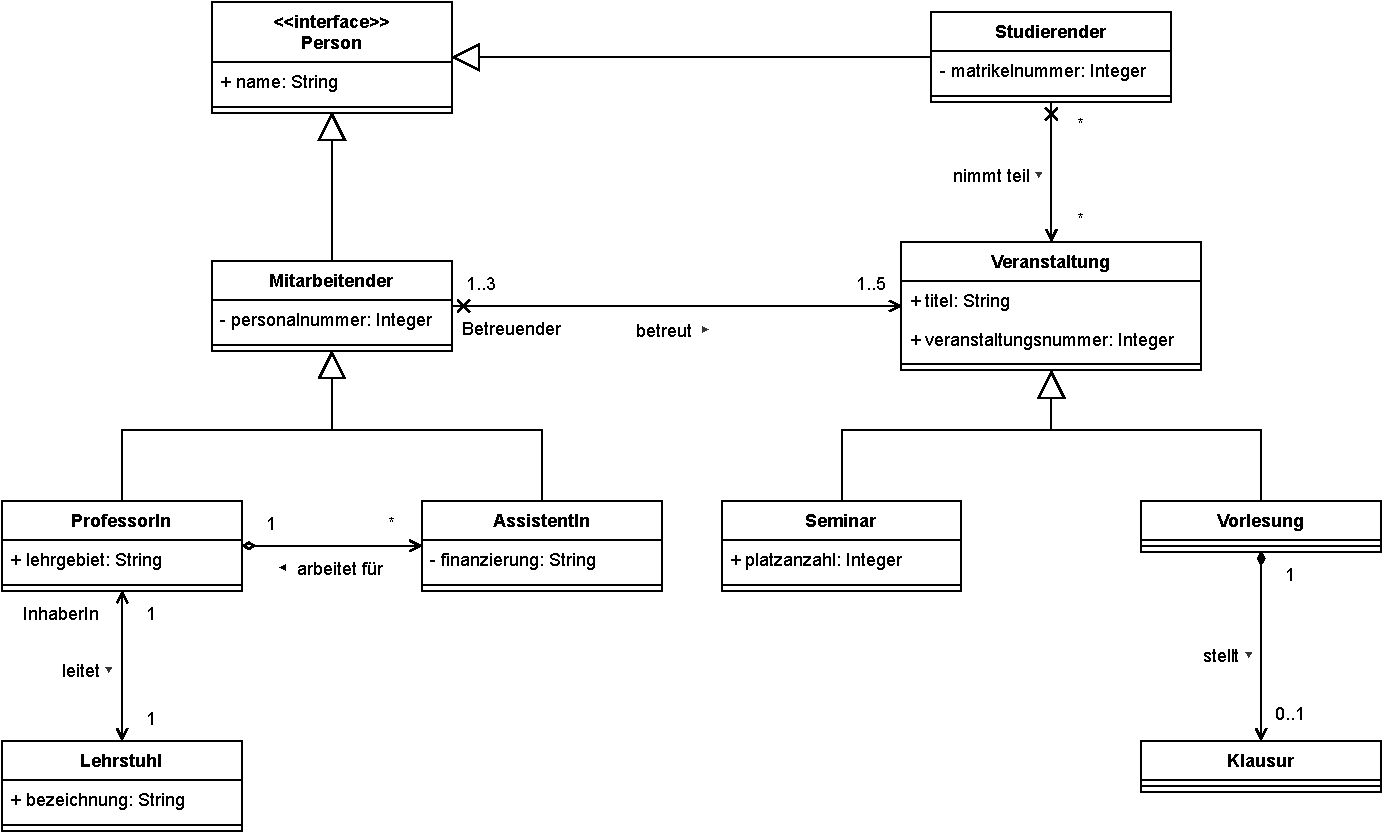
\includegraphics[width=\textwidth]{swt_wende_tim_h07_class_diagram.pdf}
        \caption{\texttt{class\_diagram}}
    \end{figure}

    \newpage    
    Finden Sie jeweils ein Beispiel, bei dem eine Aggregations- und eine Kompositionsbeziehung sinnvoll ist.
    Erläutern Sie kurz den Unterschied zwischen Aggretation und Komposition anhand des Bespiels.

    \begin{figure}[ht]
        \centering
        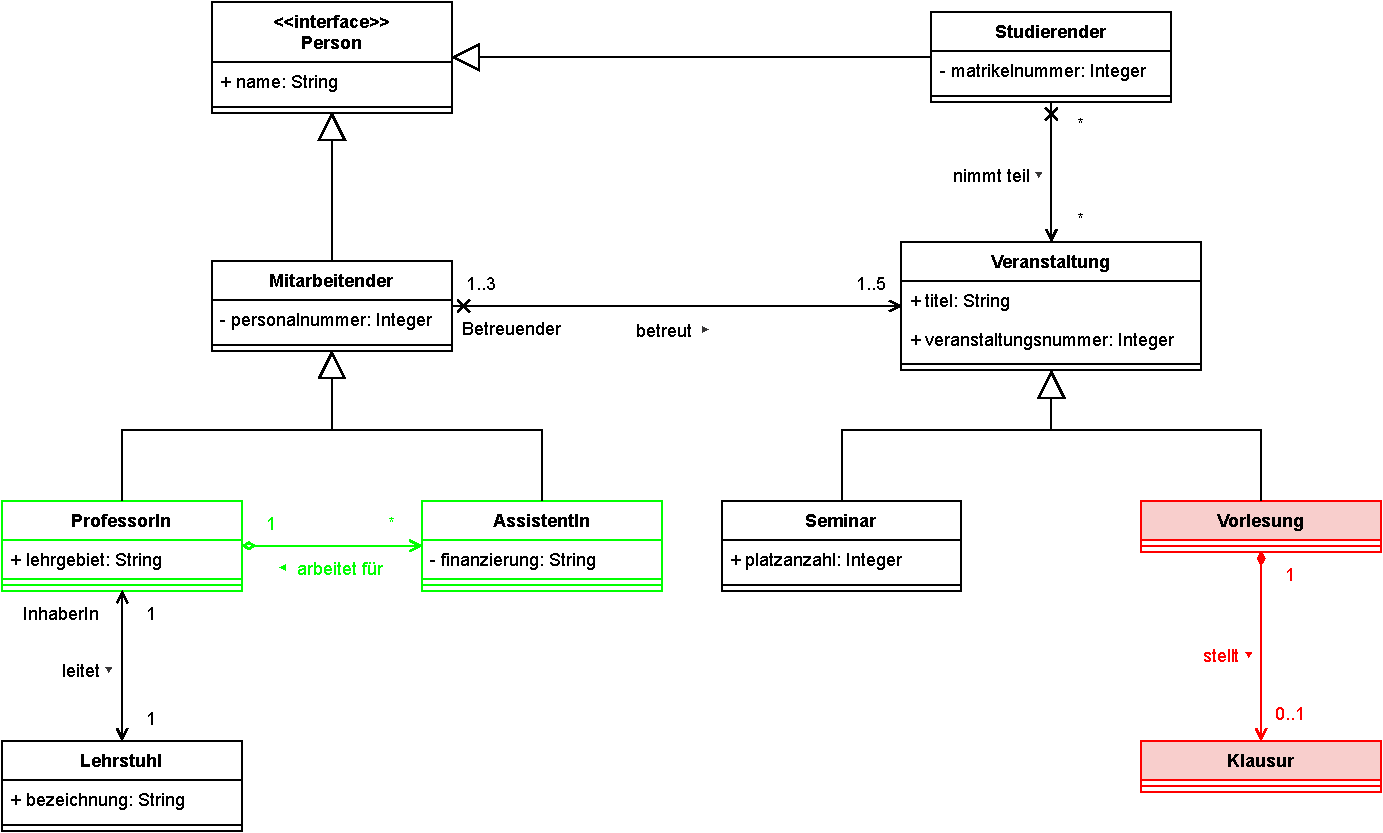
\includegraphics[width=0.75\textwidth]{swt_wende_tim_h07_class_diagram_diff.pdf}
        \caption{\texttt{class\_diagram\_diff}}
    \end{figure}

    Als Beispiel für die \textcolor{green}{Aggregation} habe ich die Beziehung zwischen \underline{ProfessorIn} und \underline{AssistentIn} gewählt.
    Im Gegensatz dazu steht die \textcolor{red}{Komposition}, welche durch die Beziehung zwischen \underline{Vorlesung} und \underline{Klausur} verkörpert wird.

    \vspace{1em}
    Einleitend fass \href{https://de.wikipedia.org/wiki/Assoziation_(UML)}{Wikipedia} es sehr gut zusammen (stark gekürzt):\\
    \textbf{Aggregation}:\\
    \gqq{Eine exakte Definition wird in der UML2 nicht gegeben [\ldots].
    Ein konkreter Nutzen lässt sich z. B. ableiten, indem man einem Ende einer Assoziation eine besondere Betonung zukommen lässt}\\
    \textbf{Komposition}:\\
    Der Unterschied zur Aggregation ist, dass ein Objekt, das als Ganzes Teile enthält, für die Existenz der Teile verantwortlich ist.

    Also anschaulich:
    \begin{figure}[ht]
        \centering
        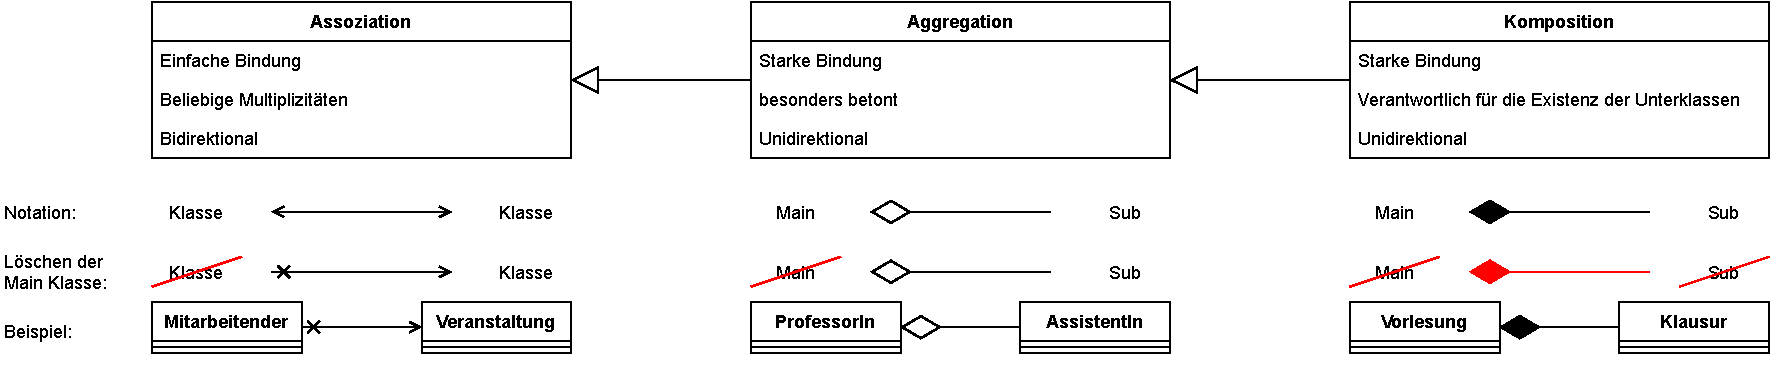
\includegraphics[width=0.75\textwidth]{swt_wende_tim_h07_class_diagram_chart.pdf}
        \caption{\texttt{class\_diagram\_chart}}
    \end{figure}

    Um diese Informationen auf unser Beispiel anzuwenden (bzg. der Klassen; nicht der Objekte):\\
    Ein/e \underline{AssistentIn} ist besonders *betont abhängig* von einem/einer \underline{ProfessorIn}.
    Diese Bindung ist beispielsweise stärker, als die Bindung eines \underline{Studierenden} zu einer \underline{Veranstaltung}, jedoch ist der/die \underline{ProfessorIn} nicht verantwortlich für die Existenz eines/einer \underline{AssistentIn}.\\
    Die \underline{Klausur} existiert jedoch ausschließlich, wenn die \underline{Vorlesung} existiert.
    Fällt diese Weg, wird das Objekt \underline{Klausur} automatisch entfernt.

    \vspace{1em}
    Anmerkungen zum Diagramm:
    \begin{itemize}
        \item Ich gehe davon aus, dass eine Klausur für nur eine Vorlesung genutzt werden kann.
            Da Dies nicht so genau aus der Aufgabenstellung erkennbar ist, sei dies hier erwähnt.
        \item Die Multiplizität am Pfeil \texttt{nimmt teil} bei \underline{Studierender} könnte auch mit Hilfe des Attributs \texttt{platzanzahl} aus \underline{Seminar} beschrieben werden.
            So könnte (um bei Java zu bleiben):\\
            \texttt{(Veranstaltung.isClass(Seminar)) ? ((Seminar) Veranstaltung).platzanzahl : *}\\
            die Genauigkeit der Obergrenze erhöhen.
    \end{itemize}

    \newpage
    \section*{Kohäsion und Kopplung}

    \begin{enumerate}
        \item Beschreiben Sie in eigenen Worten das Prinzip der Kohäsion und Kopplung in der Implementierung von Software-Projekten.

            Die Bindung verschiedener Objekte (Klassen/ Methoden/ ganzen Modulen/ \ldots), entsteht durch gegenseitige Methodenaufrufe oder Referenzen.
            Die Dichte bzw. Anzahl dieser Bindungen wird durch das Maß der Kohäsion beschrieben.
            Dieses Maß beschreibt den logischen Zusammenhang der jeweiligen Objekte.
            Die Bindung verschiedener Pakete wird Kopplung genannt.
            Man möchte die paketintern Kohäsion der Bindung also so hoch wie möglich halten, und die Bindung der verschiedenen Pakete so gering wie möglich.
        
        \item Warum sind hohe Kohäsion und lose Kopplung der niedrigen Kohäsion und enger Kopplung vorzuziehen?
        
            Wenn man seinen Code in Pakete aufteilt, möchte man paketintern einen großen logischen Zusammenhang.
            Zusätzlich möchte man so wenige Querverbindungen zwischen den Paketen wie möglich erstellen, da man sonst in Gefahr läuft, dass jede Klasse in irgend einer Art und Weise abhänhig von einer Zweiten ist.
            Wenn man zusätzlich diese bereits reduzierten Querverbindungen auf eine Schnittstelle begrenzt, kann man \gqq{hinter} dieser \gqq{Proxy}-Klasse den Code beliebig ändern, ohne, dass man andere Klassen ebenfalls ändern muss.
            Die einzige Klasse, welche beeinflusst wird, ist die \gqq{Proxy}-Klasse. So hat man nur eine (ver-)Bindung und in den Paketen eine hohe Kohäsion.

        \item Geben Sie ein \textbf{eigenes} Beispiel in Form eines Klassendiagrammes für hohe Kohäsion und lose Kopplung an.
        
            \begin{figure}[ht]
                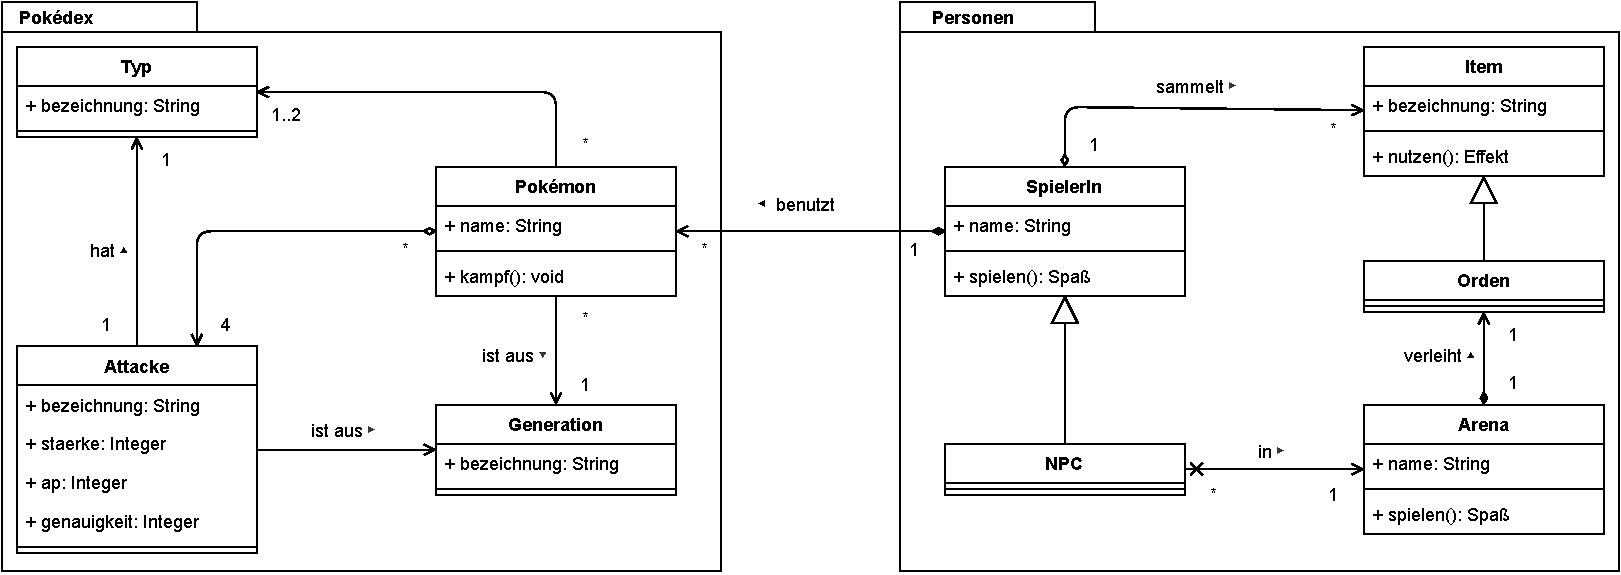
\includegraphics[width=\textwidth]{swt_wende_tim_h07_class_diagram_example.pdf}
                \caption{\texttt{class\_diagram\_example}}
            \end{figure}
    \end{enumerate}

    \newpage
    \section*{Klassendiagramm Implizierungen}

    Gegeben sei folgendes UML-Klassendiagramm mit ähnlichem Kontext wie aus der ersten Aufgabe. 

    Zusätzliche Annahmen:
    \begin{itemize}
        \item Jede Person hat nur einen Personalausweis.
            Wir vernachlässigen den Fakt, dass man diesen verlegen oder verlieren kann.
        \item Studierende können sich bei der Bibliothek auf Wartelisten für Bücher setzen lassen
        Die Bibliothek benachrichtigt die Studierenden nach dem FIFO-Prinzip, wenn das Buch verfügbar ist
        Das soll sich in der verwendeten Datenstruktur für die Assoziation zwischen Bibliothek und Studierender in der Bibliothek widerspiegeln.
    \end{itemize}

    Hinweis: Achten Sie darauf, dass die Multiplizitäten vom Code auch abgebildet werden! Zum Beispiel, dass eine Person keine Null-Referenz auf einen Personalausweis haben darf!
    
    \begin{figure}[ht]
        \centering
        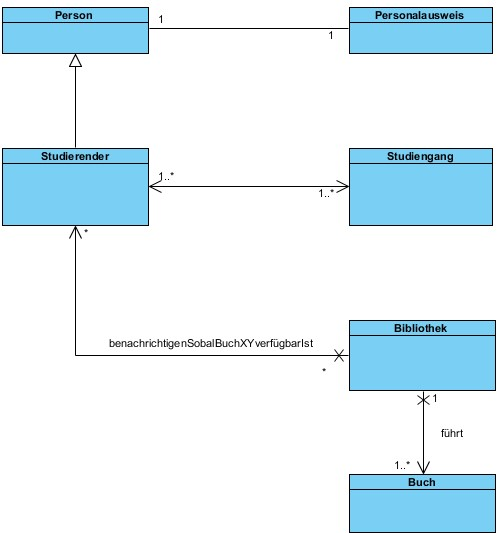
\includegraphics[width=0.4\textwidth]{class_diagram.jpg}
        \caption{\texttt{class\_diagram}}
    \end{figure}

    Tragen Sie in die vorgegebenen Java-Klassen, die Umsetzung der Assoziationen mit korrekter Multiplizität ein. An welchen Stellen ergibt es Sinn, die Assoziationen weiter über (unique, ordered) einzuschränken?
    
    Hier mein Klassendiagramm, welches nach dem Javacode erstellt wurde:

    \begin{figure}[ht]
        \centering
        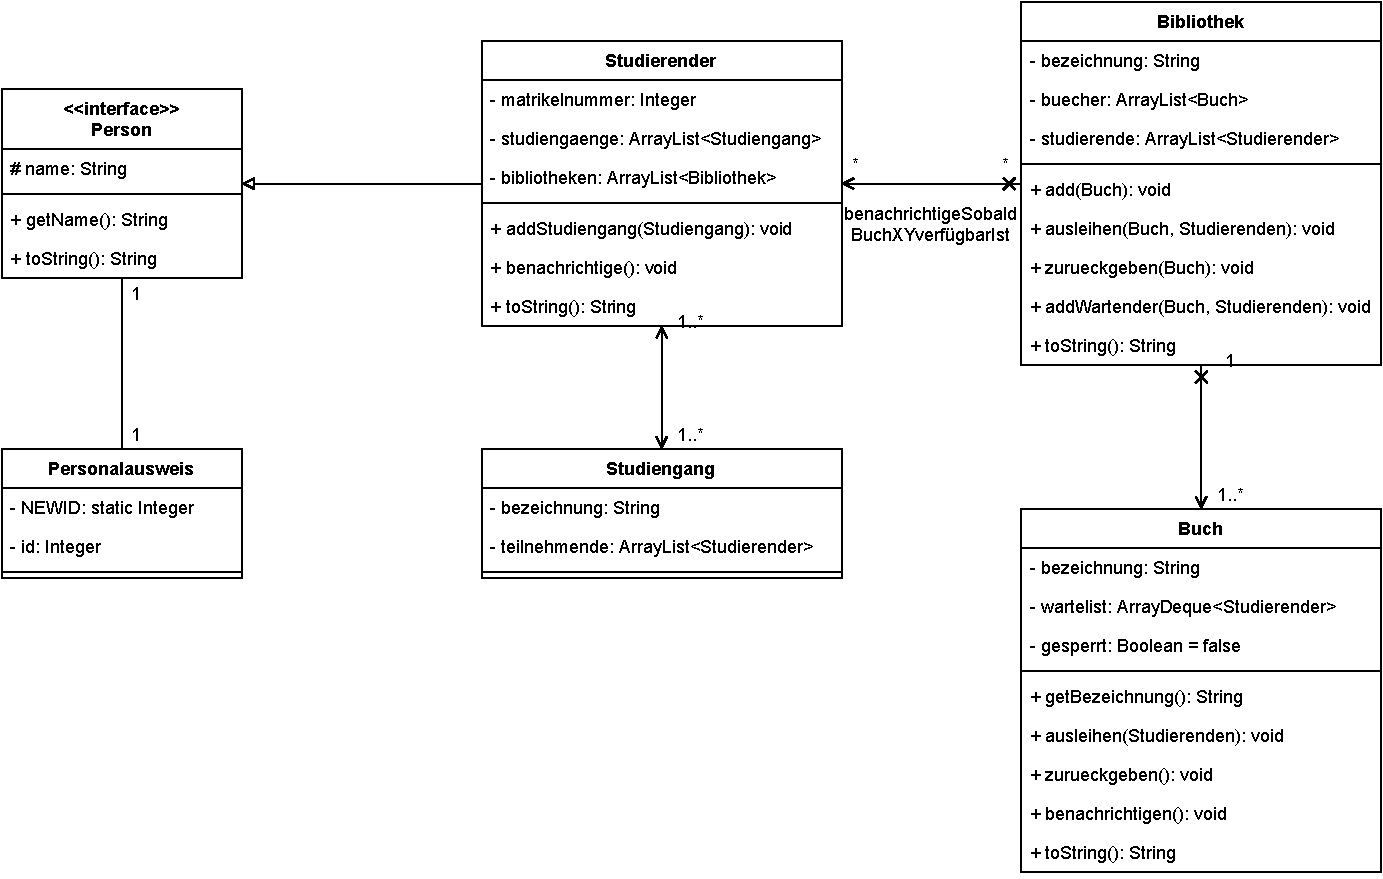
\includegraphics[width=0.75\textwidth]{swt_wende_tim_h07_class_diagram_after.pdf}
        \caption{\texttt{class\_diagram\_after}}
    \end{figure}

    \newpage
    Zuerst gebe ich aus debugging Zwecken alle erstellten Studierenden aus.
    Dann folgt das Erstellen, sowie initiales nutzen der Bibliothek.
    Und zu guter letzt werden verschiedene Methoden ausprobiert.

    Um den Code zu besser verstehen zu können, werde ich diesen nun Stück für Stück präsentieren.
    Hierzu verwende ich folgende Reihenfolge:
    
    \begin{enumerate}
        \item Output der Testklasse
        \item Klasse Test inklusive \texttt{main Methode}
        \item Klasse Studiengang
        \item Klasse Person
        \item Klasse Personalausweis
        \item Klasse Studierender
        \item Klasse Bibliothek
        \item Klasse Buch
    \end{enumerate}

    Der folgende Output wird von der \texttt{Test Klasse} erzeugt:
    
    \VerbatimInput{out.txt}

    \newpage
    Schauen wir uns dazu erstmal die \texttt{Test Klasse} an:
    \inputminted{java}{Test.java}

    \newpage
    In der ersten Zeile der \texttt{main Methode} finden wir:
    \begin{minted}{java}
        Studiengang matse = new Studiengang("Angewandte Mathematik und Informatik");
    \end{minted}

    Hier wird ein Objekt der Klasse Studiengang erstellt.
    Dieses bekommt eine Bezeichnung; hier beispielsweise \gqq{Angewandte Mathematik und Informatik}; übergeben.
    Die dazuehörige Klasse sieht wie folgt aus:

    \inputminted{java}{Studiengang.java}

    \newpage
    Schauen wir uns die \texttt{main Methode} oder \texttt{addTeilnehmender} aus \texttt{Studiengang.java} an, bemerken wir, dass wir einen Studierenden benötigen:

    \begin{minted}{java}
       Studierender tim = new Studierender("Tim Wende", 3281514, new Personalausweis(), matse);
    \end{minted}

    Der Studierende benötigt einen Namen; hier \gqq{Tim Wende}; eine Matrikelnummer, einen Personalausweis, sowie einen ersten Studiengang; hier \gqq{matse};
    Zusätzlich benötigen wir erstmal die Abstrakte Klasse \texttt{Person}, von welcher \texttt{Studierender} erben wird.

    \inputminted{java}{Person.java}

    \newpage
    Hier sehen wir eine kleine Hilfsklasse \texttt{Personalausweis}.
    Diese wird ausschließlich von der Klasse \texttt{Person} genutzt:

    \inputminted{java}{Personalausweis.java}

    \newpage
    Nun, wie versprochen \texttt{Studierender.java}:

    \inputminted{java}{Studierender.java}

    \newpage
    Als nächstes wird in der \texttt{main Methode} eine Bibliothek erstellt.
    Diese trägt den kreativen Namen \gqq{RWTH Bib}:
    
    \begin{minted}{java}
        Bibliothek rwthbib = new Bibliothek("RWTH Bib");
    \end{minted}

    Da die Klasse \texttt{Bibliothek} als \gqq{Proxy}-Klasse gebraucht wird (siehe 2.2), leitet sie mehrere Funktionen \gqq{dumm} weiter. Diese werden also meistens auf dem Objekt selber ausgeführt:

    \inputminted{java}{Bibliothek.java}

    \newpage
    Nun erstellen wir ein paar Bücher und fügen sie unserer Bibliothek hinzu.
    Als Buchnamen mussten alte Hausaufgaben von mir herhalten.
    Teilweise werden die Bücher direkt vorgemerkt.

    \begin{minted}{java}
        rwthbib.addBuch(new Buch("swt_wende_tim_h01.pdf"));
    \end{minted}

    \inputminted{java}{Buch.java}

    Diese werden nun teilweise vorgemerkt:
    
    \begin{minted}{java}
		rwthbib.addWartender(h05, tim);
    \end{minted}

    ausgeliehen:
    
    \begin{minted}{java}
		rwthbib.ausleihen(h05, tim); // gesperrt
    \end{minted}

    oder zurückgegeben:
    
    \begin{minted}{java}
		rwthbib.zurueckgeben(h05); // entsperrt
    \end{minted}

    Die zugehörigen Ausgaben sind in \texttt{out.txt} zu finden.

    \end{document}